%%%%%%%%%%%%%%%%%%%%%%%%%%%%%%%%%%%%%%%%%
% Arsclassica Article
% LaTeX Template
% Version 1.1 (1/8/17)
%
% This template has been downloaded from:
% http://www.LaTeXTemplates.com
%
% Original author:
% Lorenzo Pantieri (http://www.lorenzopantieri.net) with extensive modifications by:
% Vel (vel@latextemplates.com)
%
% License:
% CC BY-NC-SA 3.0 (http://creativecommons.org/licenses/by-nc-sa/3.0/)
%
%%%%%%%%%%%%%%%%%%%%%%%%%%%%%%%%%%%%%%%%%

%----------------------------------------------------------------------------------------
%	PACKAGES AND OTHER DOCUMENT CONFIGURATIONS
%----------------------------------------------------------------------------------------

\documentclass[
10pt, % Main document font size
a4paper, % Paper type, use 'letterpaper' for US Letter paper
oneside, % One page layout (no page indentation)
%twoside, % Two page layout (page indentation for binding and different headers)
headinclude,footinclude, % Extra spacing for the header and footer
BCOR5mm, % Binding correction
]{scrartcl}

%%%%%%%%%%%%%%%%%%%%%%%%%%%%%%%%%%%%%%%%%
% Arsclassica Article
% Structure Specification File
%
% This file has been downloaded from:
% http://www.LaTeXTemplates.com
%
% Original author:
% Lorenzo Pantieri (http://www.lorenzopantieri.net) with extensive modifications by:
% Vel (vel@latextemplates.com)
%
% License:
% CC BY-NC-SA 3.0 (http://creativecommons.org/licenses/by-nc-sa/3.0/)
%
%%%%%%%%%%%%%%%%%%%%%%%%%%%%%%%%%%%%%%%%%

%----------------------------------------------------------------------------------------
%	REQUIRED PACKAGES
%----------------------------------------------------------------------------------------

\usepackage[
nochapters, % Turn off chapters since this is an article        
beramono, % Use the Bera Mono font for monospaced text (\texttt)
eulermath,% Use the Euler font for mathematics
pdfspacing, % Makes use of pdftex’ letter spacing capabilities via the microtype package
dottedtoc % Dotted lines leading to the page numbers in the table of contents
]{classicthesis} % The layout is based on the Classic Thesis style

\usepackage{arsclassica} % Modifies the Classic Thesis package

\usepackage[T1]{fontenc} % Use 8-bit encoding that has 256 glyphs

\usepackage[utf8]{inputenc} % Required for including letters with accents

\usepackage{graphicx} % Required for including images
\graphicspath{{Figures/}} % Set the default folder for images

\usepackage{enumitem} % Required for manipulating the whitespace between and within lists

\usepackage{lipsum} % Used for inserting dummy 'Lorem ipsum' text into the template

\usepackage{subfig} % Required for creating figures with multiple parts (subfigures)

\usepackage{amsmath,amssymb,amsthm} % For including math equations, theorems, symbols, etc

\usepackage{varioref} % More descriptive referencing

\usepackage{csvsimple} % Used for tables

\usepackage{float}

\usepackage{placeins}

\usepackage{chngpage}

%----------------------------------------------------------------------------------------
%	THEOREM STYLES
%---------------------------------------------------------------------------------------

\theoremstyle{definition} % Define theorem styles here based on the definition style (used for definitions and examples)
\newtheorem{definition}{Definition}

\theoremstyle{plain} % Define theorem styles here based on the plain style (used for theorems, lemmas, propositions)
\newtheorem{theorem}{Theorem}

\theoremstyle{remark} % Define theorem styles here based on the remark style (used for remarks and notes)

%----------------------------------------------------------------------------------------
%	HYPERLINKS
%---------------------------------------------------------------------------------------

\hypersetup{
%draft, % Uncomment to remove all links (useful for printing in black and white)
colorlinks=true, breaklinks=true, bookmarks=true,bookmarksnumbered,
urlcolor=webbrown, linkcolor=RoyalBlue, citecolor=webgreen, % Link colors
pdftitle={}, % PDF title
pdfauthor={\textcopyright}, % PDF Author
pdfsubject={}, % PDF Subject
pdfkeywords={}, % PDF Keywords
pdfcreator={pdfLaTeX}, % PDF Creator
pdfproducer={LaTeX with hyperref and ClassicThesis} % PDF producer
} % Include the structure.tex file which specified the document structure and layout

\hyphenation{Fortran hy-phen-ation} % Specify custom hyphenation points in words with dashes where you would like hyphenation to occur, or alternatively, don't put any dashes in a word to stop hyphenation altogether

%----------------------------------------------------------------------------------------
%	TITLE AND AUTHOR(S)
%----------------------------------------------------------------------------------------

\title{\normalfont\spacedallcaps{Predicting Heart Disease Mortality}} % The article title

%\subtitle{Subtitle} % Uncomment to display a subtitle

\author{\spacedlowsmallcaps{Carlos Alberto Nava Fonseca\textsuperscript{1}}} % The article author(s) - author affiliations need to be specified in the AUTHOR AFFILIATIONS block

\date{} % An optional date to appear under the author(s)

%----------------------------------------------------------------------------------------

\begin{document}

%----------------------------------------------------------------------------------------
%	HEADERS
%----------------------------------------------------------------------------------------

\renewcommand{\sectionmark}[1]{\markright{\spacedlowsmallcaps{#1}}} % The header for all pages (oneside) or for even pages (twoside)
%\renewcommand{\subsectionmark}[1]{\markright{\thesubsection~#1}} % Uncomment when using the twoside option - this modifies the header on odd pages
\lehead{\mbox{\llap{\small\thepage\kern1em\color{halfgray} \vline}\color{halfgray}\hspace{0.5em}\rightmark\hfil}} % The header style

\pagestyle{scrheadings} % Enable the headers specified in this block

%----------------------------------------------------------------------------------------
%	TABLE OF CONTENTS & LISTS OF FIGURES AND TABLES
%----------------------------------------------------------------------------------------

\maketitle % Print the title/author/date block

\setcounter{tocdepth}{2} % Set the depth of the table of contents to show sections and subsections only

\tableofcontents % Print the table of contents

\listoffigures % Print the list of figures

\listoftables % Print the list of tables

%----------------------------------------------------------------------------------------
%	ABSTRACT
%----------------------------------------------------------------------------------------

\section*{Executive Summary} % This section will not appear in the table of contents due to the star (\section*)

The present report documents the techniques and analysis of the rate of heart disease (per 100,000 individuals) across the United States at the county-level from socioeconomic indicators. The data is taken from the United States Department of Agriculture Economic Research Service (USDA ERS) and the University of Wisconsin Population Health Institute. County Health Rankings \& Roadmaps.

There are 33 variables in this dataset. Each row in the dataset represents a United States county that is unidentifiable in the dataset. While all the variables were studied, the discoveries lead to detect outliers, lack of data and wrong values. During the data processing, education and health variables were the most significantly correlated to the heart disease mortality. And, after using categories for some variables, both area information about the county and the economic typology play a major role in the prediction of heart disease.

When developing the Machine Learning model, only one model couldn't get an effective prediction. Therefore Stacking Regressions were used to improve accuracy.

%----------------------------------------------------------------------------------------
%	AUTHOR AFFILIATIONS
%----------------------------------------------------------------------------------------

\let\thefootnote\relax\footnotetext{\textsuperscript{1} \textit{navafoseca.carlos@gmail.com}}

%----------------------------------------------------------------------------------------

%\newpage % Start the article content on the second page, remove this if you have a longer abstract that goes onto the second page

%----------------------------------------------------------------------------------------
%	INTRODUCTION
%----------------------------------------------------------------------------------------

\section{Introduction}

This chapter describes the dataset used to develop a Machine Learning model to predict Heart Disease. These datasets (training and test sets) were obtained from the United States Department of Agriculture Economic Research Service (USDA ERS).

\subsection{Data Exploration: Target Variable}

From the dataset provided, there are 33 variables, which are divided into four categories:
\begin{itemize}
    \item Area: variables that contain information about the county
    \item Economic Indicators: they are categories of economic dependence, labour force, unemployment and insurance
    \item Health: indicators about obesity, smoking, diabetes and other characteristics of the county's population
    \item Demographics: information from the county's characteristics such as age percentage distribution, education, and others.
\end{itemize}

Also, additional information was given from the article from Jones (2009) \cite{Jones2009} on relevant factors of heart disease linked with the rural population with certain economic characteristics.

The variable selected for prediction is: heart\_disease\_mortality\_per\_100k. It is defined as the rate of heart disease (per 100,000 individuals) across the data set. A brief summary of the variable is presented in Table~\ref{tab:sum_01}.

\FloatBarrier 
 \begin{table}[]
 	\caption{Statistical Summary of Heart Disease Mortality per 100k} \label{tab:sum_01}
 	\begin{tabular}{llllll} 
 		\hline
 		& count  & mean   & std   & min   & max   \\ \hline
 		\textbf{heart\_disease\_mortality\_per\_100k} & 3198.0 & 279.37 & 58.95 & 109.0 & 512.0 \\ \hline
 	\end{tabular}
 \end{table}

From Table~\ref{tab:sum_01} it can be seen that the target variable main statistics. Plotting this variable it is observable in Figure~\ref{fig:target_01} that is near a normal distributed variable and negatively skewed (slightly pointing to the left).

\FloatBarrier
\begin{figure}[H]
\centering 
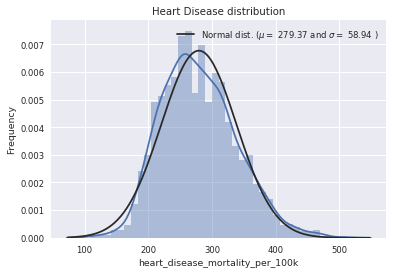
\includegraphics[width=0.75\columnwidth]{heart_normal_01.png} 
\caption[Target Variable]{Target Variable Distribution vs Theoretical Normal Distribution (\emph{Own elaboration made with: Python Seaborn}), \index{Heart Disease distribution.}}
\label{fig:target_01} 
\end{figure}

The Q–Q (quantile-quantile) plot helps to compare the two probability distributions by plotting their quantiles against each other. As seen in Figure~\ref{fig:prob_01} it is presented the graphically the properties of the normal distribution and the variable distribution. This Q–Q plot compares a sample of data on the vertical axis to a statistical population on the horizontal axis. The points follow a linear pattern, suggesting that the data are not distributed as a standard normal $X ~ N(0,1)$. Fortunately, there is little offset between the line and the points suggest that the data follows a $X ~ N(\mu,\sigma)$ distribution. 

\FloatBarrier
\begin{figure}[H]
\centering 
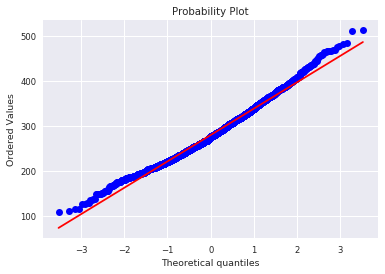
\includegraphics[width=0.75\columnwidth]{probability_plot_01.png} 
\caption[Q-Q Graph]{Probability Distribution vs Theoretical Probability Distribution (\emph{Own elaboration made with: Python Seaborn}), \index{Heart Disease probability distribution.}}
\label{fig:prob_01} 
\end{figure}

Since the target variable is left-skewed, it was transformed this variable and make it more normally distributed using the $log(1+x)$ function to be accurate in the floating-point accuracy. This skewed data is being normalised by adding one (in order to transform the 0 since $log 0$ is not defined) and taking the natural logarithm. The data can be nearly normalised using this transformation technique. Actually, many of the algorithms to be tested assume that the data is normal and calculate with this assumption. So, if data is closer to normal, the better it fits linear models.

After the logarithmic transformation of the target variable, it was obtained Figure~\ref{fig:target_02} with almost no skew suggesting that the data appears more normally distributed.

\FloatBarrier
\begin{figure}[H]
\centering 
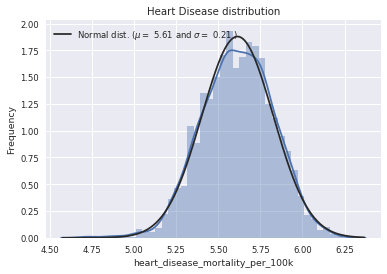
\includegraphics[width=0.75\columnwidth]{heart_normal_02.png} 
\caption[Target Variable Normalized]{Target Variable Distribution vs Theoretical Normal Distribution (\emph{Own elaboration made with: Python Seaborn}), \index{Heart Disease distribution.}}
\label{fig:target_02} 
\end{figure}

In Figure~\vref{fig:prob_02}, it details the gap between the theoretical an data distribution are closer confirming that the logarithmic transformation normalized the data making it suitable to use linear modelling.

\FloatBarrier
\begin{figure}[H]
\centering 
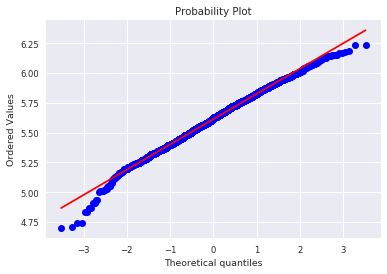
\includegraphics[width=0.75\columnwidth]{probability_plot_02.png} 
\caption[Q-Q Graph Normalized]{Probability Distribution vs Theoretical Probability Distribution (\emph{Own elaboration made with: Python Seaborn}), \index{Heart Disease probability distribution.}}
\label{fig:prob_02} 
\end{figure}

\subsection{Data Exploration: Train Variables}

From the data there are 3198 samples, which can be used to train model; also 33 features and 1 target variable. A brief summary of non-categorical data is presented in Table~\ref{tab:sum_02}. It can be seen that most data is normalized since it is presented in terms of ratio per one hundred or percentage. Some data from the Health category (air pollution, homicides per 100,000 inhabitants, vehicle crash per 100,000 inhabitants, population per dentist and population per physician) are not normalized. This represents an advantage now that the target data is normalized.

\begin{table}[]
\small
\begin{adjustwidth}{-.5in}{-.5in}
\caption{Statistical Summary of Variables Description} \label{tab:sum_02}
\begin{tabular}{llllll}
\hline
                                                          & count & mean    & std     & min  & max    \\ \hline
econ\_\_pct\_civilian\_labor                              & 3198  & 0.47    & 0.07    & 0.21 & 1      \\
econ\_\_pct\_unemployment                                 & 3198  & 0.06    & 0.02    & 0.01 & 0.25   \\
econ\_\_pct\_uninsured\_adults                            & 3196  & 0.22    & 0.07    & 0.05 & 0.5    \\
econ\_\_pct\_uninsured\_children                          & 3196  & 0.09    & 0.04    & 0.01 & 0.28   \\ \hline
demo\_\_pct\_female                                       & 3196  & 0.5     & 0.02    & 0.28 & 0.57   \\
demo\_\_pct\_below\_18\_years\_of\_age                    & 3196  & 0.23    & 0.03    & 0.09 & 0.42   \\
demo\_\_pct\_aged\_65\_years\_and\_older                  & 3196  & 0.17    & 0.04    & 0.04 & 0.35   \\
demo\_\_pct\_hispanic                                     & 3196  & 0.09    & 0.14    & 0    & 0.93   \\
demo\_\_pct\_non\_hispanic\_african\_american             & 3196  & 0.09    & 0.15    & 0    & 0.86   \\
demo\_\_pct\_non\_hispanic\_white                         & 3196  & 0.77    & 0.21    & 0.05 & 0.99   \\
demo\_\_pct\_american\_indian\_or\_alaskan\_native        & 3196  & 0.02    & 0.08    & 0    & 0.86   \\
demo\_\_pct\_asian                                        & 3196  & 0.01    & 0.03    & 0    & 0.34   \\
demo\_\_pct\_adults\_less\_than\_a\_high\_school\_diploma & 3198  & 0.15    & 0.07    & 0.02 & 0.47   \\
demo\_\_pct\_adults\_with\_high\_school\_diploma          & 3198  & 0.35    & 0.07    & 0.07 & 0.56   \\
demo\_\_pct\_adults\_with\_some\_college                  & 3198  & 0.3     & 0.05    & 0.11 & 0.47   \\
demo\_\_pct\_adults\_bachelors\_or\_higher                & 3198  & 0.2     & 0.09    & 0.01 & 0.8    \\
demo\_\_birth\_rate\_per\_1k                              & 3198  & 11.68   & 2.74    & 4    & 29     \\
demo\_\_death\_rate\_per\_1k                              & 3198  & 10.3    & 2.79    & 0    & 27     \\ \hline
health\_\_pct\_adult\_obesity                             & 3196  & 0.31    & 0.04    & 0.13 & 0.47   \\
health\_\_pct\_adult\_smoking                             & 2734  & 0.21    & 0.06    & 0.05 & 0.51   \\
health\_\_pct\_diabetes                                   & 3196  & 0.11    & 0.02    & 0.03 & 0.2    \\
health\_\_pct\_low\_birthweight                           & 3016  & 0.08    & 0.02    & 0.03 & 0.24   \\
health\_\_pct\_excessive\_drinking                        & 2220  & 0.16    & 0.05    & 0.04 & 0.37   \\
health\_\_pct\_physical\_inacticity                       & 3196  & 0.28    & 0.05    & 0.09 & 0.44   \\
health\_\_air\_pollution\_particulate\_matter             & 3170  & 11.63   & 1.56    & 7    & 15     \\
health\_\_homicides\_per\_100k                            & 1231  & 5.95    & 5.03    & -0.4 & 50.49  \\
health\_\_motor\_vehicle\_crash\_deaths\_per\_100k        & 2781  & 21.13   & 10.49   & 3.14 & 110.45 \\
health\_\_pop\_per\_dentist                               & 2954  & 3431.43 & 2569.45 & 339  & 28130  \\
health\_\_pop\_per\_primary\_care\_physician              & 2968  & 2551.34 & 2100.46 & 189  & 23399  \\
\hline
\end{tabular}
\end{adjustwidth}
\end{table}

Further analysis of the data presented in Table~\ref{tab:sum_02} suggest that the variables might be correlated with each other. To graphically test this hypothesis, it is visualized as the correlations between variables in Figure~\ref{fig:correlation_01}.
 

\FloatBarrier
\begin{figure}[H]
\centering 
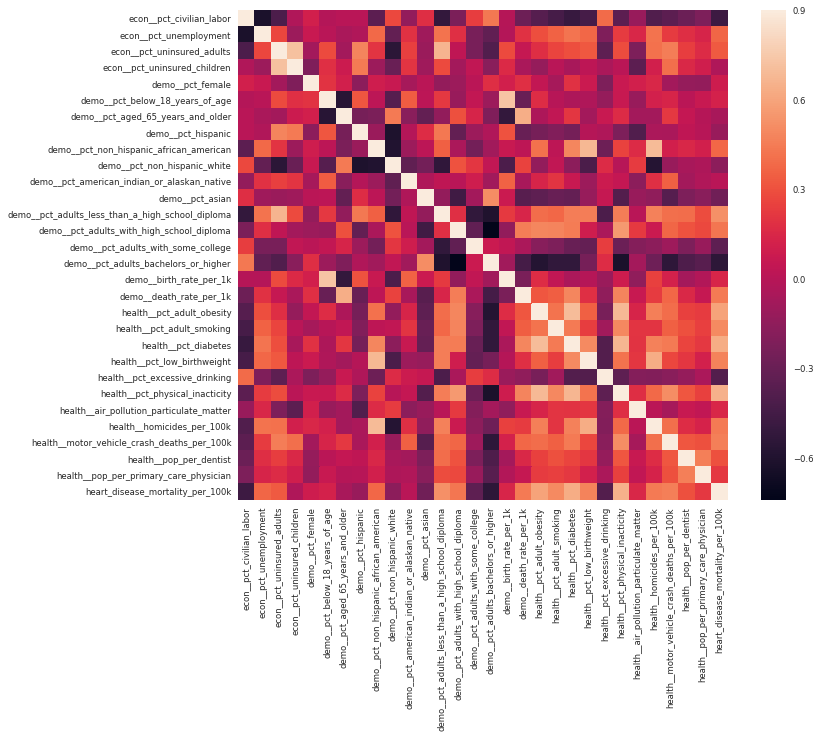
\includegraphics[width=0.8\columnwidth]{correlation_01.png} 
\caption[Correlation Heat Map]{Correlation Heat Map (\emph{Own elaboration made with: Python Seaborn}), \index{Correlation between variables.}}
\label{fig:correlation_01} 
\end{figure}

From this Figure, the assumption is that the lower right side of the graph holds more correlation to the target variable. There are also negative correlations, mainly from labour and education. Further detail on variables correlated with more than $|0.5|$ with the target variable was plotted in the following Figure~\ref{fig:correlation_02}.

\FloatBarrier
\begin{figure}[H]
\centering 
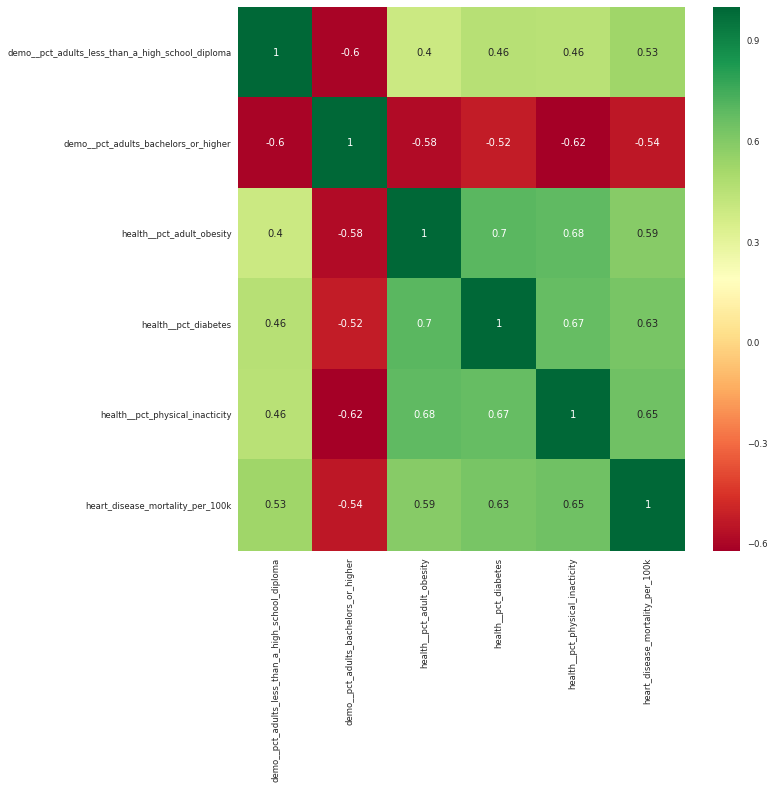
\includegraphics[width=0.7\columnwidth]{correlation_02.png} 
\caption[Detailed Correlation Heat Map]{Detailed Correlation Heat Map (\emph{Own elaboration made with: Python Seaborn}), \index{Correlation between variables $<|0.5|$.}}
\label{fig:correlation_02} 
\end{figure}

These findings suggest that the lifestyle factors that come with income can reduce or increase the risk for heart disease. With this in mind its logic to think that factors like education, income and wealth play an important role in overall health. Social position can influence a person’s behaviour, impacting decisions related to diet, exercise and smoking.

Exploring the data in more detail, the analysis proceeds to the data set distribution. Presented in Figure~\ref{fig:boxplot_01} that data has many outliers and is not normally distributed.

\FloatBarrier
\begin{figure}[H]
\centering 
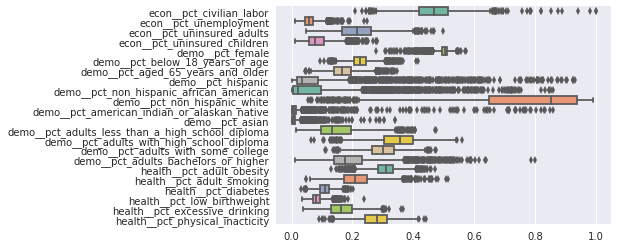
\includegraphics[width=0.9\columnwidth]{box_plot_01.png} 
\caption[Box plot of data variables]{Percentage Variables (\emph{Own elaboration made with: Python Seaborn}), \index{Data Variables Boxplot}}
\label{fig:boxplot_01} 
\end{figure}

A closer look to data which is $<|0.5|$ correlated to the target variable (see Figure~\ref{fig:boxplot_02}) follows the same pattern. Therefore the model must be aware of the skewness of each variable and some of these variables might have outliers. From this analysis, the conclusion is that the mean of each variable presented in Table~\ref{tab:sum_02} as part of the statistical description, is sensitive to these outliers if they are removed or transformed.

\FloatBarrier
\begin{figure}[H]
\centering 
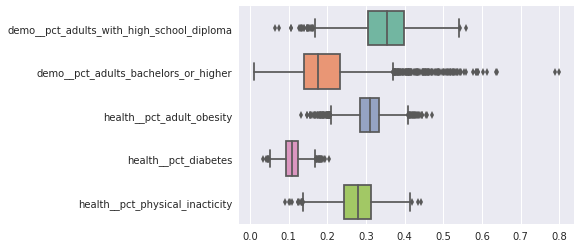
\includegraphics[width=0.9\columnwidth]{box_plot_02.png} 
\caption[Box plot of correlated data variables]{Percentage Variables with $<|0.5|$ correlation (\emph{Own elaboration made with: Python Seaborn}), \index{Data Variables Boxplot}}
\label{fig:boxplot_02} 
\end{figure}

\subsection{Missing Data and Skewness}

Missing values in the training data set can affect the prediction or classification of a model negatively. Also, some machine learning algorithms can't accept missing data. Take for example Support Vector Machines or Linear Regression.

Having understood a general perspective on how data variables have some correlation role with the target variable, and a brief description of them, the following procedures are made to the the data variables. After the review the data composition in Table~\ref{tab:data_01} that there is lack of data ranging from $60.48\%$ to $0.16\%$ which must be treated in order to try different models without errors.

\begin{table}[]
\small
\caption{Missing Data Percentage} \label{tab:data_01}
\centering
\begin{tabular}{ll}
\hline
                                                   & Missing Ratio \\ \hline
health\_\_homicides\_per\_100k                     & 60.481        \\
health\_\_pct\_excessive\_drinking                 & 29.277        \\
health\_\_pct\_adult\_smoking                      & 13.794        \\
health\_\_motor\_vehicle\_crash\_deaths\_per\_100k & 12.138        \\
health\_\_pop\_per\_dentist                        & 7.04          \\
health\_\_pop\_per\_primary\_care\_physician       & 6.594         \\
health\_\_pct\_low\_birthweight                    & 5.241         \\
health\_\_air\_pollution\_particulate\_matter      & 1.051         \\
health\_\_pct\_adult\_obesity                      & 0.159         \\
health\_\_pct\_diabetes                            & 0.159         \\
health\_\_pct\_physical\_inacticity                & 0.159         \\
...												  & ...           \\
demo\_\_pct\_aged\_65\_years\_and\_older           & 0.159         \\
\hline
\end{tabular}
\end{table}

From the previous section, it is known that data mean is sensitive. Therefore, it must take into account that the gaps in the data set must consider both the training and testing sets and go through the same procedure. Having known that the mean is sensitive, the median was considered to fill the missing values on variables who were below 1\% of missing data.

The other variables received different treatment. Since data were missing between 5 to 60.5 per cent, the approach was to use normalized data within the range of the mean and one standard deviation. In other words, a sample random variable $X$ with $N(\mu,\sigma)$ was used to fill the missing values.

Additionally, categorical variables must be mapped to account them in the analysis. The following data variables were mapped according to their characteristics:

\begin{itemize}
\item \textit{area\_\_rucc} will be mapped between Metropolitan Counties (Value: 1) and Non-Metropolitan Counties (Value: 0).
\item \textit{area\_\_urban\_influence} will be mapped between Large influence (Value: 1) and Small influence (Value: 0).
\item \textit{econ\_\_economic\_typology} will be mapped between economic activities that are classified as stressful (manufacturing, government dependent and mining) with value of 1, others will be non-stressful (Value:0).
\item \textit{yr} will be mapped according to \textit{a} as 1 and \textit{b} as 0.
\end{itemize}

Also, based on the correlation analysis and the mapped variables some elements were dropped since they could not be transformed in normalized data or had not a direct approach to heart disease. Homicides, crash deaths, and population per dentist and physicians were left out.

To make all data normally distributed, the skew for each data variable was calculated. Values for the first 10 variables are presented in Table~\ref{tab:skew_01}. 

\begin{table}[]
\small
\caption{Skew Value in Data} \label{tab:skew_01}
\centering
\begin{tabular}{ll}
\hline
                                                   & Skew  \\ \hline
demo\_\_pct\_american\_indian\_or\_alaskan\_native & 7.78  \\
demo\_\_pct\_asian                                 & 7.338 \\
demo\_\_pct\_hispanic                              & 3.182 \\
demo\_\_pct\_non\_hispanic\_african\_american      & 2.282 \\
area\_\_urban\_influence                           & 2.104 \\
demo\_\_pct\_adults\_bachelors\_or\_higher         & 1.515 \\
health\_\_pct\_low\_birthweight                    & 1.23  \\
econ\_\_pct\_unemployment                          & 1.195 \\
econ\_\_pct\_uninsured\_children                   & 1.19  \\
demo\_\_birth\_rate\_per\_1k                       & 0.951 \\
...												  & ...   \\
\hline
\end{tabular}
\end{table}

The assumption of normality at the beginning of this analysis leads to modelling that is simple, mathematically tractable, and powerful compared to tests that do not make the normality assumption. Unfortunately, the skewed data set is in fact not approximately normal. However, an appropriate transformation of a data set can often yield a data set that does follow approximately a normal distribution. This increases the applicability and usefulness of models based on the normality assumption.

The Box-Cox transformation is a particularly useful family of transformations. It is defined as:

\begin{equation}
T(Y) = (Y^{\lambda} - 1)/\lambda
\label{eq:boxcox}
\end{equation}

where Y is the response variable and $\lambda$ is the transformation parameter. For $\lambda = 0$, the natural log of the data is taken instead of using the Formula~\ref{eq:boxcox}. Variables with an absolute value of skewness greater than $0.75$ were transformed with a $\lambda = 0.15$.

The process that leads to normalizing the data in the training set was also used in the test set so it can predict with the assumptions made for the variables.

%----------------------------------------------------------------------------------------
%	METHODS
%----------------------------------------------------------------------------------------

\section{Machine Learning Model}

Breiman (1996)~\cite{Breiman1996} presents stacking regressions is a method for forming linear combinations of different predictors to give improved prediction accuracy. The idea is to use cross-validation data and least squares under non-negativity constraints to determine the coefficients in the combination. The idea was first presented by Wolpert (1992)~\cite{Wolpert1992}. Under this idea, a model was developed.

\subsection{Base Models} 

The following models were tested:

\begin{enumerate}
\item LASSO Regression. 
\item Elastic Net Regression. 
\item Gradient Boosting Regression. 
\item Extreme Gradient Boosting (or XGBoost).
\end{enumerate}

The models were evaluated by their performance using cross-validation of the Root Mean Squared Logarithmic Error (RMSLE) error. The following results were obtained:

\begin{table}[]
\small
\caption{Base Models Results} \label{tab:base_models}
\centering
\begin{tabular}{lll}
\hline
                         & Mean   & Std.     \\ \hline
Lasso score:             & 0.1194 & (0.0030) \\
ElasticNet score:        & 0.1193 & (0.0030) \\
Kernel Ridge score:      & 0.1262 & (0.0040) \\
Gradient Boosting score: & 0.0991 & (0.0032) \\
Xgboost score:           & 0.1067 & (0.0032) \\
\hline
\end{tabular}
\end{table}

Now that the procedure has the Mean and Standard Deviation, the first approach is averaging base models. Obtaining the following result: \\ \textbf{Averaged base models score: Mean = 0.1113 Std. = (0.0034)}.

When stacking the averaged models as a meta-model, it got: \\ \textbf{Stacking Averaged models score: Mean = 0.1000 Std. = (0.0036)}.

Finally, after and creating a stacked classification model we used the exponential function on the predicted model. Obtaining the results in the original scale for submission.


%----------------------------------------------------------------------------------------
%	RESULTS AND DISCUSSION
%----------------------------------------------------------------------------------------

\section{Results and Conclusions}

The analysis presented in this report acknowledge the following findings:

\begin{itemize}
\item Filling the missing values with mean/median/mode for a high rate of present data (over 99\%) do not generate outliers and is appropriate for data close to a normal distribution.
\item In some variables, random sampling was used to predict missing values using a random variable with $X ~ N(\mu,\sigma)$ distribution.
\item Categorical variables were mapped in binary values to include them in the model.
\item After filling the missing data and mapping the categorical variables, the skewness of the data was modelled with the Box-Cox technique to adjust them into normalized data.
\item After the classification with base models, a stacking regression model was used to predict the values of the target variable.
\end{itemize}

Based on the Root Mean Squared Logarithmic Error (RMSLE), the model constructed for predicting the heart disease using a stacking regression showed to perform better than the base models alone.

Further work can be implemented with the categorical data and missing data with other techniques such as Decision Trees based on correlated variables.

%----------------------------------------------------------------------------------------
%	BIBLIOGRAPHY
%----------------------------------------------------------------------------------------

\renewcommand{\refname}{\spacedlowsmallcaps{References}} % For modifying the bibliography heading

\bibliographystyle{unsrt}

\bibliography{sample.bib} % The file containing the bibliography

%----------------------------------------------------------------------------------------

\end{document}